\documentclass[11pt]{article}
\usepackage[T1]{fontenc}
\usepackage[english,polish]{babel}
\usepackage{amsmath}
\usepackage{fancyhdr}
\usepackage{graphicx}
\usepackage{wrapfig}
\usepackage{cite}
\usepackage{colortbl}
\DeclareMathOperator{\tg}{tg}
\newcommand{\tgx}{\tg x}
\title{Skoki narciarskie}
\author{Damian Górski}
\begin{document}
\maketitle
\noindent
\newpage
\tableofcontents
\newpage
Skoki narciarskie to sport sezonowy. Charakteryzuje się bardzo dużą popularnością wśród Polaków, ponieważ jako jeden z nielicznych sportów posiada polskich reprezentantów, którzy radzą sobie bardzo dobrze na arenie międzynarodowej. W skrócie przedstawię ciekawostki oraz aktualne wyniki naszych sportowców.
\section{Zasady}
\subsection{Punktacja}
Zawodnik zostaje klasyfikowany według punktów uzyskanych za skok. Punkty zdobywa za: 
\begin{itemize}
\item punkty za odległość - długość skoku mierzona jest od progu skoczni do pięty tylnego buta w chwili zetknięcia się narty ze stokiem z dokładnością do 0.5 metra
\item noty za styl - skok oceniany przez pięciu sędziów, przy czym najwyższa i najniższa nota się nie liczy. Reszta jest dodawana (możliwe oceny - od 0 do 20 punktów).
\item bonus - punkty dodawane lub odejmowane ze względu na warunki pogodowe oraz za zmianę platformy startowej
\end{itemize}
Te trzy rzeczy składają się na sumę punktów uzyskanych przez skoczka za jego lot.
\subsection{Sprzęt}
Każdy zawodnik musi ściśle przestrzegać określonych zasad do których sędziowie podchodzą rygorystycznie.
\begin{itemize}
\item narty - nie mogą być dłuższe niż 146\% wzrostu zawodnika a ich szerokość nie przekraczać 105 mm
\item wiązania - powinny odpiąć buty od narty podczas upadku, co zmniejsza ryzyko kontuzji. Powinny również znajdować się w odległości 57\% całej narty od jej początku.
\item buty - Nie powinny ograniczać ruchów stopy zawodnika jak i również utrzymać ją w odpowiednim położeniu, wykonane ze skóry.
\item kombinezon - grubość max 5 mm, rozmiar ma być równy wymiarom zawodnika (mierzone w miejscach: udo, klatka piersiowa, obwód w pasie, obwód ramienia).
\item kask
\item gogle
\item rękawice
\end{itemize}
\subsection{Przedskoczek}
Przedskoczek jest to osoba, która nie uczestniczy w zawodach i przed rozpoczęciem konkursu testuje daną skocznie. W szczególnie jest on wykorzystywany do testowania skoczni w trudnych warunkach, ale także testuje nowe skocznie czy obiekty, które były poddane modernizacji. Jednym z ich zadań jest pomoc jury w dobraniu odpowiedniej długości rozbiegu. Skaczą oni również w przerwach między seriami, by przetrzeć zalegający na rozbiegu śnieg.
\newline 
\newline \textit{{\small Ciekawostka: Przedskoczkami są zazwyczaj starsi już utytułowani skoczkowie, który zakończyli już swoją sportową karierę. W 1964 roku podczas Turnieju Czterech Skoczni w Garmisch-Partenkirchen przed oficjalnym rozpoczęciem konkursu oddał honorowy skok Stanisław Marusarz - miał wówczas 51 lat. }}
\subsection{Startowanie zawodników}
Po licznych sporach w 2010 roku ustalono, że pomimo zielonego światła, jeżeli trener zauważy niebezpieczeństwo albo warunki atmosferyczne niepozwalające na oddanie dobrego skoku, może on je wyłączyć. Jednak następną możliwość do oddania skoku wyznacza jury i nie oddanie skoku będzie egzekwowane jako dyskwalifikacja.
\newpage
\subsection{Punkty}
Punkty przyznane zawodnikowi za zdobyte miejsce w konkursach \\pod egidą FIS (International Ski Federation) \textit{\small patrz: Tablica 1 oraz Tablica 2}
\begin{table}
\caption{Punktacja}
\begin{center}
\begin{tabular}{|c|l|l|l|l|l|l|l|l|l|l|l|l|l|l|l|}
\hline Miejsce & 1. & 2. & 3. & 4. & 5. & 6. & 7. & 8. & 9. & 10. & 11. & 12. & 13. & 14. & 15. \\ \hline \hline
Punkty & 100 & 80 & 60 & 50 & 45 & 40 & 36 & 32 & 29 & 26 & 24 & 22 & 20 & 18 & 16 \\ \hline
\end{tabular}
\end{center}
\end{table}
\begin{table}
\caption{Punktacja c.d}
\begin{center}
\begin{tabular}{|c|l|l|l|l|l|l|l|l|l|l|l|l|l|l|l|}
\hline Miejsce & 16. & 17. & 18. & 19. & 20. & 21. & 22. & 23. & 24. & 25. & 26. & 27. & 28. & 29. & 30.  \\ \hline \hline
Punkty & 15 & 14 & 13 & 12 & 11 & 10 & 9 & 8 & 7 & 6 & 5 & 4 & 3 & 2 & 1 \\ \hline
\end{tabular}
\end{center}
\end{table}
\\\\
\arrayrulecolor{red}\doublerulesepcolor{blue}
Natomiast w konkursach drużynowych punktacja wygląda w trochę inny sposób (\textit{\small patrz: Tablica 3})
\begin{table}
\caption{Punktacja drużynowa}
\begin{center}
\begin{tabular}{|c|l|l|l|l|l|l|l|l|}
\hline Miejsce & 1. & 2. & 3. & 4. & 5. & 6. & 7. & 8. \\ \hline \hline
Punkty & 400 & 350 & 300 & 250 & 200 & 150 & 100 & 50 \\ \hline
\end{tabular}
\end{center}
\end{table}
\section{Zawody}\label{zawody}
Najważniejsze zawody dla skoczków narciarskich to: 
\begin{itemize}
\item Igrzyska Olimpijskie - co 4 lata (ostatnie w 2018 roku)
\item Mistrzostwa Świata w skokach narciarskich - co 2 lata, w lata nieparzyste (ostatnie w 2017 roku)
\item Mistrzostwa Świata w lotach narciarskich - co 2 lata, w lata parzyste (ostatnie w 2018 roku)
\item Turniej Czterech Skoczni - odbywany co rocznie
\item Puchar Świata w skokach narciarskich - odbywany co rocznie
\item Letnie Grand Prix - odbywany co rocznie
\end{itemize}
\newpage
\section{Najdalsze skoki narciarskie na świecie}
Przez lata dokumentowane były skoki oddane przez zawodników. Z roku na rok odległości są co raz dłuższe co świadczy o ciągłym rozwijaniu się tego sportu.
\\\\
Powyżej znajdują się wybrane rekordy świata w danym roku \\(\textit{\small patrz: Tablica 4})
\begin{table}
\caption{Rekordy świata}
\begin{center}
\begin{tabular}{|c|l|l|l|l|l|}
\hline Lp. & rok & rekordzista & kraj & miejsce & odległość \\ \hline \hline
1. & 1808 & Olaf Rye & Norwegia & Eidsberg & 9,5 m \\ 
2. & 1900 & Olaf Tandberg & Norwegia & Bærum & 35,5 m \\
3. & 1931 & Bronisław Czech & Polska & Ponte di Legno & 79,5 m \\
4. & 1938 & Josef Bradl & Austria & Planica & 107,0 m \\
5. & 1967 & Kjell Sjöberg & Szwecja & Oberstdorf & 148,0 m \\
6. & 1984 & Matti Nykänen & Finlandia & Oberstdorf & 185,0 m \\
7. & 2003 & Matti Hautamäki & Finlandia & Planica & 231,0 m \\
8. & 2015 & Peter Prevc & Słowenia & Vikersund & 250,0 m \\
9. & 2017 & Stefan Kraft & Austria & Vikersund & 253,5 m \\
\hline
\end{tabular}
\end{center}
\end{table}
\section{Polska a skoki narciarskie}
\subsection{Indywidualni reprezentanci}
Aktualnymi skoczkami reprezentującymi nasz kraj na arenie międzynarodowej są:
\begin{itemize}
\item Kamil Stoch
\item Piotr Żyła
\item Maciej Kot
\item Dawid Kubacki
\item Stefan Hula
\item Jakub Wolny
\end{itemize}
\newpage
\noindent
Szczególną postacią w tym zestawieniu jest zdecydowanie Kamil Stoch\\(\textit{\small patrz: Rysunek 1})\label{kamil_stoch}
\begin{wrapfigure}{r}{0.5\textwidth}
\begin{flushleft}
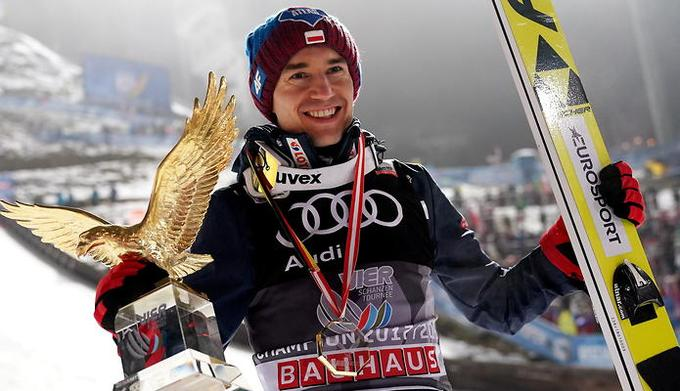
\includegraphics[angle=45,width=0.48\textwidth]{Kamil.jpg}
\end{flushleft}
\caption{Podpis}
\label{Etykieta}
\end{wrapfigure}
\\
Kamil Wiktor Stoch - (ur. 25 maja 1987 rok w Zakopanem) Polski skoczek narciarski, czterokrotny olimpijczyk. Trzykrotny indywidualny mistrz olimpijski (dwukrotnie utytułowany w 2014 roku oraz raz w 2018 roku), mistrz świata w 2013 roku, drużynowy mistrz świata z 2017 roku, dwukrotny brązowy medalista mistrzostwa świata ( 2013 rok i 2015 rok ), indywidualny srebrny i drużynowy brązowy medalista mistrzostw świata w lotach narciarskich z 2018 roku, dwukrotny drużynowy wicemistrz świata juniorów (w 2004 roku i 2005 roku), dwukrotny zdobywca Pucharu Świata (w sezonach 2013/2014 i 2017/2018), zwycięzca 65. i 66. Turnieju Czterech Skoczni (patrz: \ref{zawody}).
Nie są to jego wszystkie osiągnięcia. Stoch po raz pierwszy stanął na podium w 2011 roku w rodzinnym Zakopanem. W ramach Pucharu Świata zwyciężył w 31 konkursach, 59 razy zaś stawał na podium. Naszego najlepszego skoczka cechuje wysoka estetyka lotu jak i lądowania, przez co często zdobywa tak trudne do otrzymania "20" jury.
\subsection{Drużyna Narodowa}
Skoki narciarskie to sport w którym Polska znajduje się na bardzo wysokim miejscu w porównaniu z innymi sportami. Nasi zawodnicy indywidualnie są na bardzo wysokim poziomie, co przekłada się na świetne osiągnięcia drużynowe.
Aktualnie nasza drużyna znajduje się na pierwszym miejscu w Pucharze Narodów w skokach narciarskich w sezonie 2018/2019. 
\newpage 
\begin{center}
\begin{tabular}{||c|c|c||} \hline
\multicolumn{2}{||c||}{Kombinacja zawodników}
\\ \hline \hline
(22,22) & (11,29) \\
(24,1) & (42,2) \\ \hline
(3,1) & (3,2) \\
(44,1) & (44,2) \\ \hline
(32,2) & (22,3) \\ \hline
\end{tabular}
\end{center}
\begin{figure}
\begin{flushleft}
\caption{Polska drużyna}
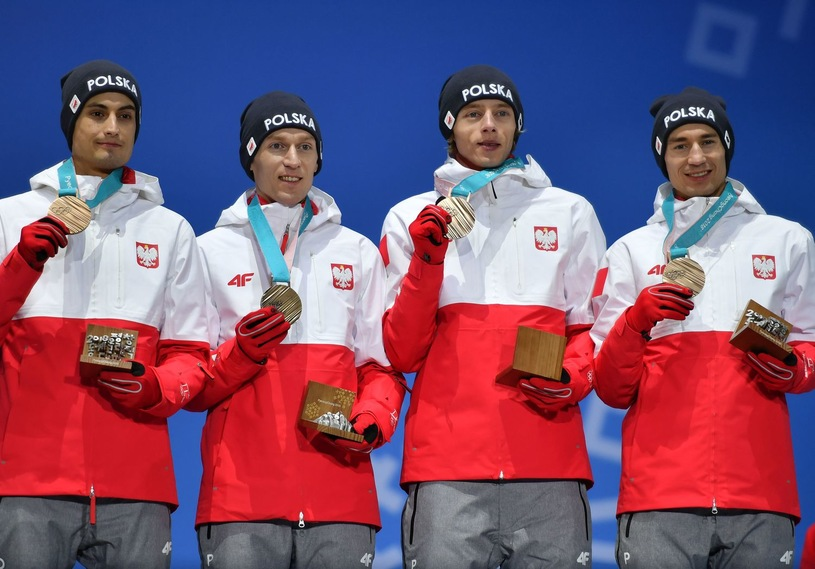
\includegraphics[width=100mm,height=!]{Druzyna.jpg}
\end{flushleft}
\end{figure}
Taka kombinacja świetnych zawodników stawia nasz kraj w bardzo korzystnym świetle, dzięki któremu mówi się o naszej reprezentacji w całej Europie.
(\textit{\small patrz: Rysunek 2}) \cite{wiki}
\newpage
\section{Ciekawostki}
\subsection{Czynnik wiatru}
Podczas wszystkich konkursów używany jest wzór matematyczny, który wyznacza czynnik wiatru podczas lotu zawodnika:
\begin{equation}
\Delta w = \tg(v) * [(s-36)/20]
\end{equation}
Gdzie:
\\
$tg(v)$ - prędkość wiatru w m/s
\\
s - długość stoku w m
\\\\
W ten sposób otrzymujemy współczynnik wiatru, który jest używany do obliczenia rzeczywistej długości skoku.
\\
Przykład:
\\
Skok długości 119.5 m na skoczni długości 130 m , wskaźnik wiatru wskazuje 1.55 m/s w plecy
\\\\
\begin{center}
$\Delta w = 1.55*[(130-36)/20]=7.28$
\end{center}
Otrzymany wynik zaokrąglamy do 0.5 m a więc nasz $\Delta w = 7.5$
\\
Po czym dodajemy otrzymany wynik do uzyskanego skoku
\\
$119.5$ m $+ 7.5$ m $= 127$ m
\subsection{Kamil Stoch i jego sekretne skupienie}
Można by się zastanawiać, dlaczego Kamil Stoch jest zawsze tak bardzo skupiony przed skokiem? Jak on to robi? Przecież nie zawsze jest się w stanie skupić w 100\% nad tym co się robi.
\\
Odpowiedź nie jest jednoznaczna, ale legendy głoszą że nasz najlepszy zawodnik (patrz: \ref{kamil_stoch}) przed każdym skokiem rozwiązuje trudne zagadnienia matematyczne które pozwalają mu się wyciszyć i skupić na skoku.
\\
Udało na się znaleźć niektóre z nich. \cite{lamport94}
\\
\begin{equation}
J_\alpha (x)=\sum_{k=0}^{\infty}\frac{(-1)^k(\frac{x}{2})^{2k+\alpha}}{k!\Gamma(k+\alpha+1)}
\end{equation}
\begin{equation}
\int\frac{\Gamma^x(n)}{x^n}dx=\Gamma^x(n)\sum_{k=1}^{n}\frac{(-ln(\Gamma(n)))^{k-1}}{x^{n-k}\prod_{i=1}^{k}(i-n)}+C
\end{equation}
\begin{equation}
\frac{1-\sin x+\sin^2 x+\sin^3 x...+(-1)^n\sin^n x+...}{1+\sin x+sin^2 x+sin^3 x+...+\sin^n x+...}=\tg^2 x
\end{equation}
\newpage
\pagecolor{red}
\listoftables
\listoffigures
\begin{thebibliography}{9}
\bibitem{lamport94}
Leslie Lamport,
\emph{\LaTeX: A Document Preparation System}.
Addison Wesley, Massachusetts,
2nd Edition,
1994.
\bibitem{wiki}
{Alur, R. and Dill, D.},
{A theory of timed automata},
{Theoretical Computer Science},
{1994},
{126},
{2},
{183-235}
\end{thebibliography}

\end{document}

